%% Introduction
\section{Methods}
%An overview of the physical components in the setup is shown in \autoref{fig:SystemOverview}.
%\autoref{fig:SystemOverview} shows a head fitted with an ANC headphone using a reference microphone (1), a headphone loudspeaker (2), an error microphone (3) and a DSP (4).

Using \autoref{fig:SystemOverview} as the outline, the DSP(4) is expanded into \autoref{fig:ANCFeedforward}.

%\begin{figure}[H]
%	\centering
%	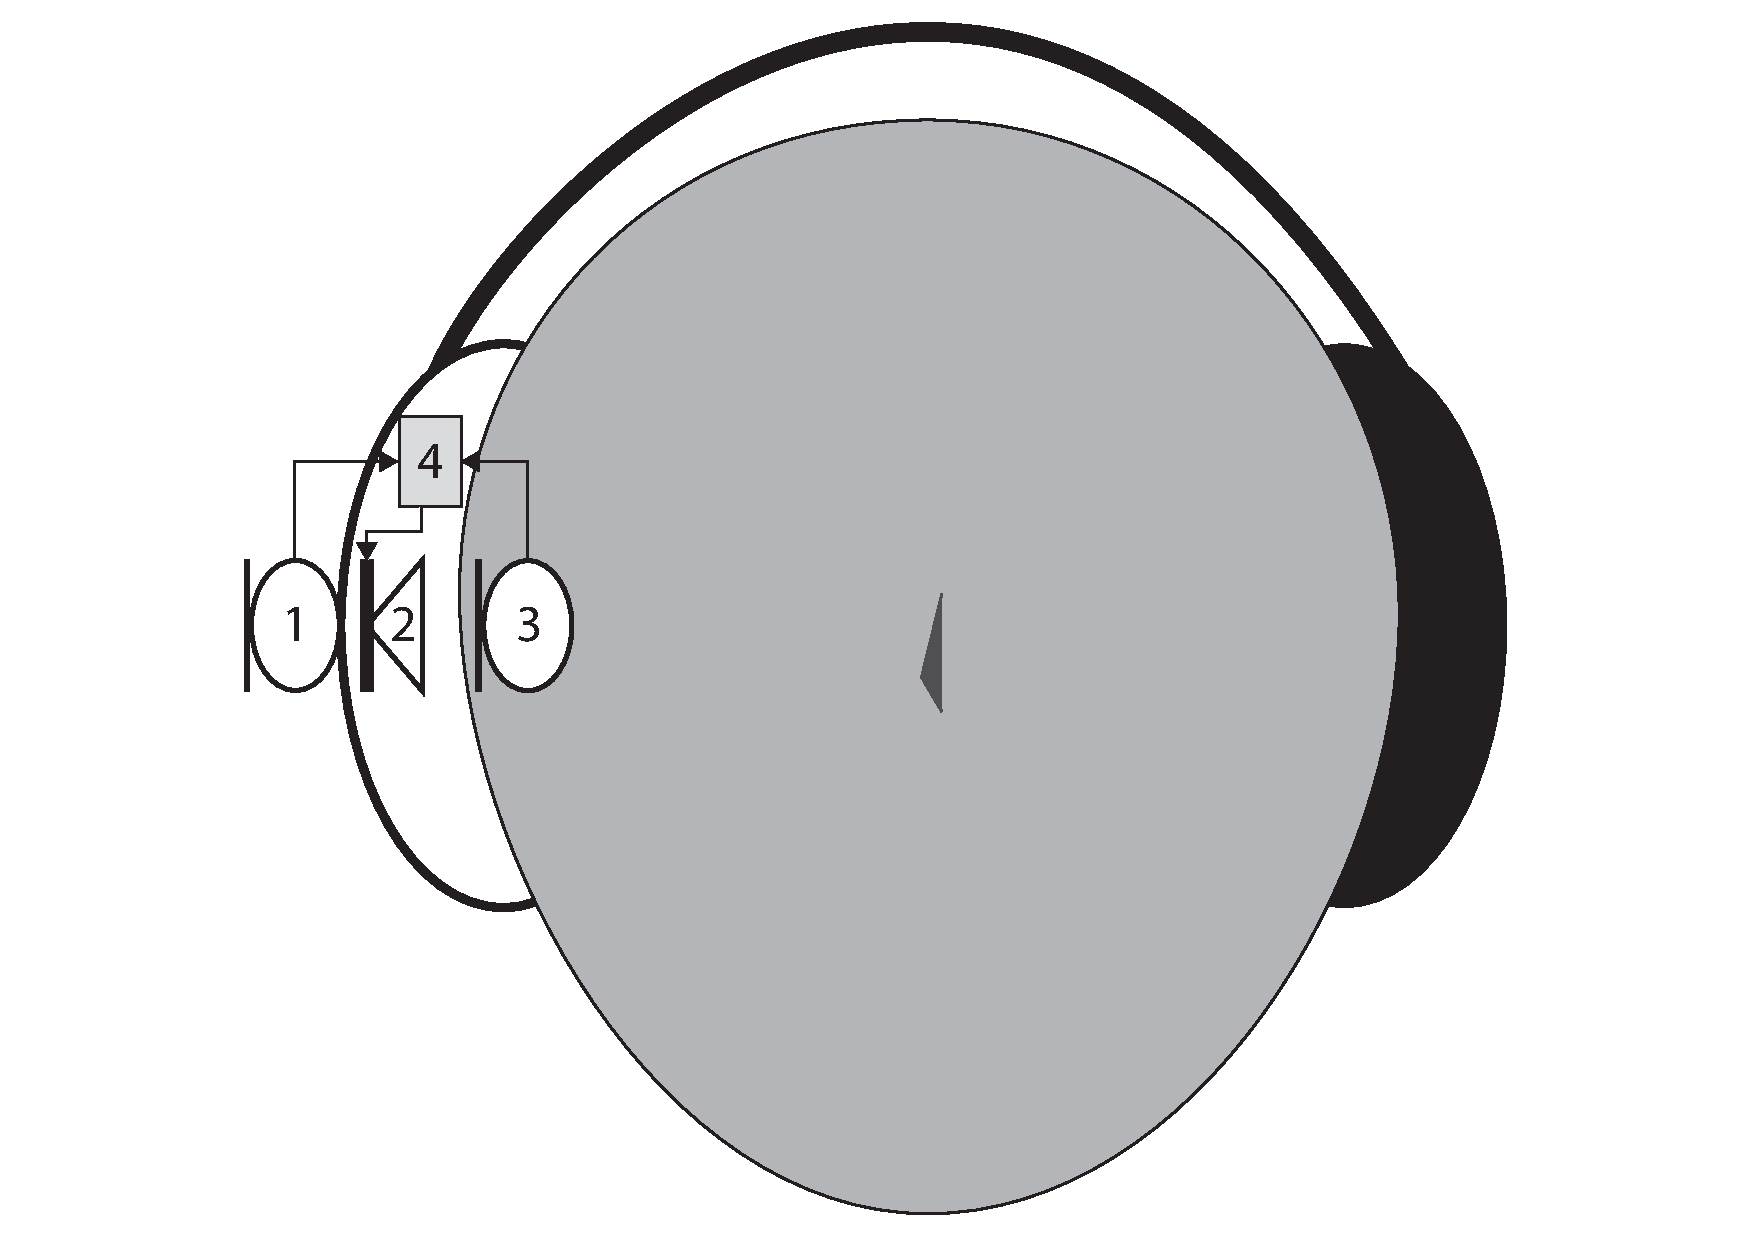
\includegraphics[width=1\columnwidth]{figures/ArticleIllustrations/SystemOverview}
%	\caption{System Overview}
%	\label{fig:SystemOverview}
%\end{figure}



\subsection{Feedforward ANC using FXLMS}
%The adaptive feedforward ANC system is shown on \autoref{fig:ANCFeedforward}


The system in \autoref{fig:ANCFeedforward} outputs a control signal $y[n]$, which ideally is a counter-phase signal of the noise. The signal is generated by inputting the reference signal $x[n]$ into a control filter consisting of adaptive coefficients $b[z]$ representing the transfer function from the reference microphone to the headphone loudspeaker. The coefficients are adapted using the FXLMS algorithm. The FXLMS algorithm inputs the filtered reference $f[n]$ signal along with the error signal $e[n]$. The filtered reference signal is used combined with the error signal to determine new optimal coefficients for the control filter, this is shown in equation \ref{eq:FXLMS}. The signals from (1)(3) are converted to the digital domain using an ADC and anti aliasing filters (AA) before processing. When processed, the output $y[n]$ is reconstructed and converted using a DAC.

 \vspace{-4mm}
{
	%\centering
	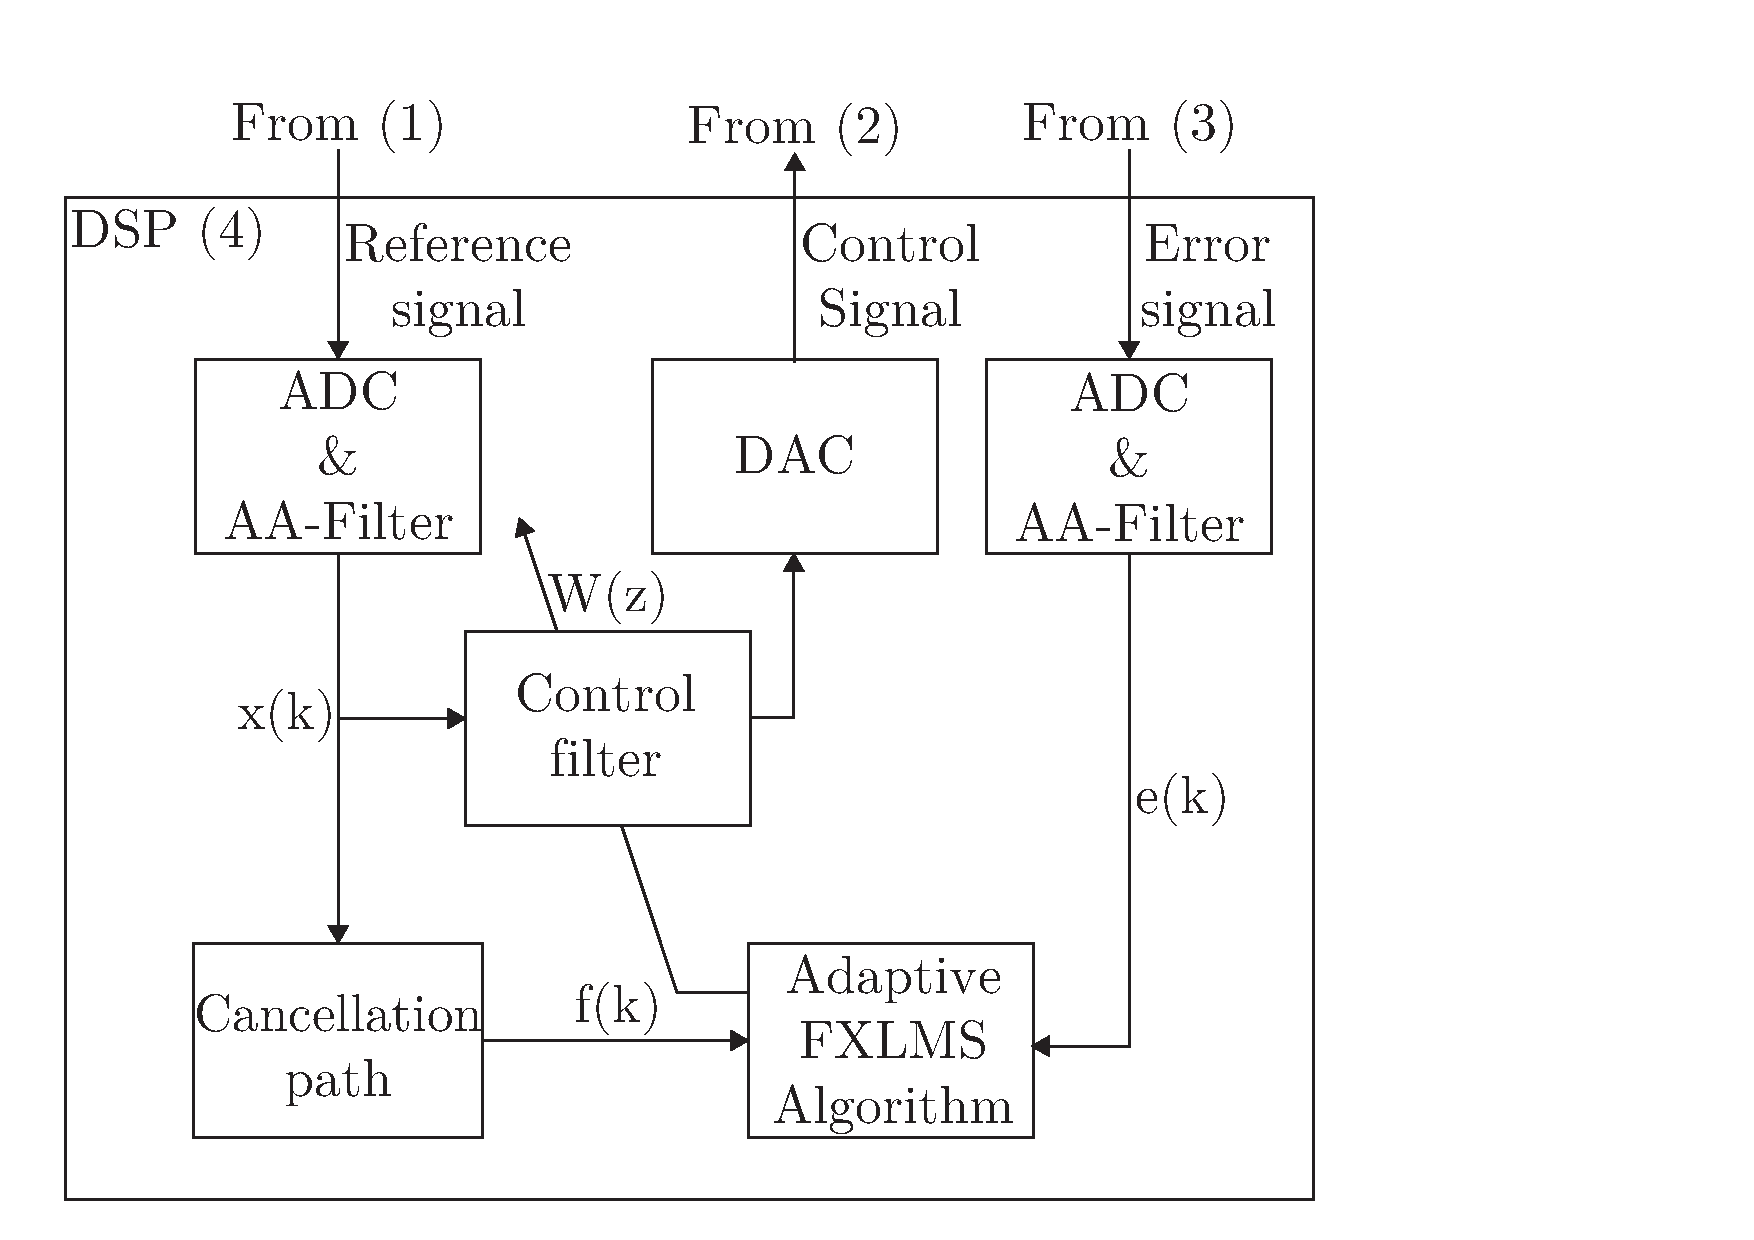
\includegraphics[width=1\columnwidth]{figures/ArticleIllustrations/ANCFeedForward}
	\captionof{figure}{Adaptive feedforward ANC system.}
	\label{fig:ANCFeedforward}
}

%\begin{figure}[H]
%	\centering
%	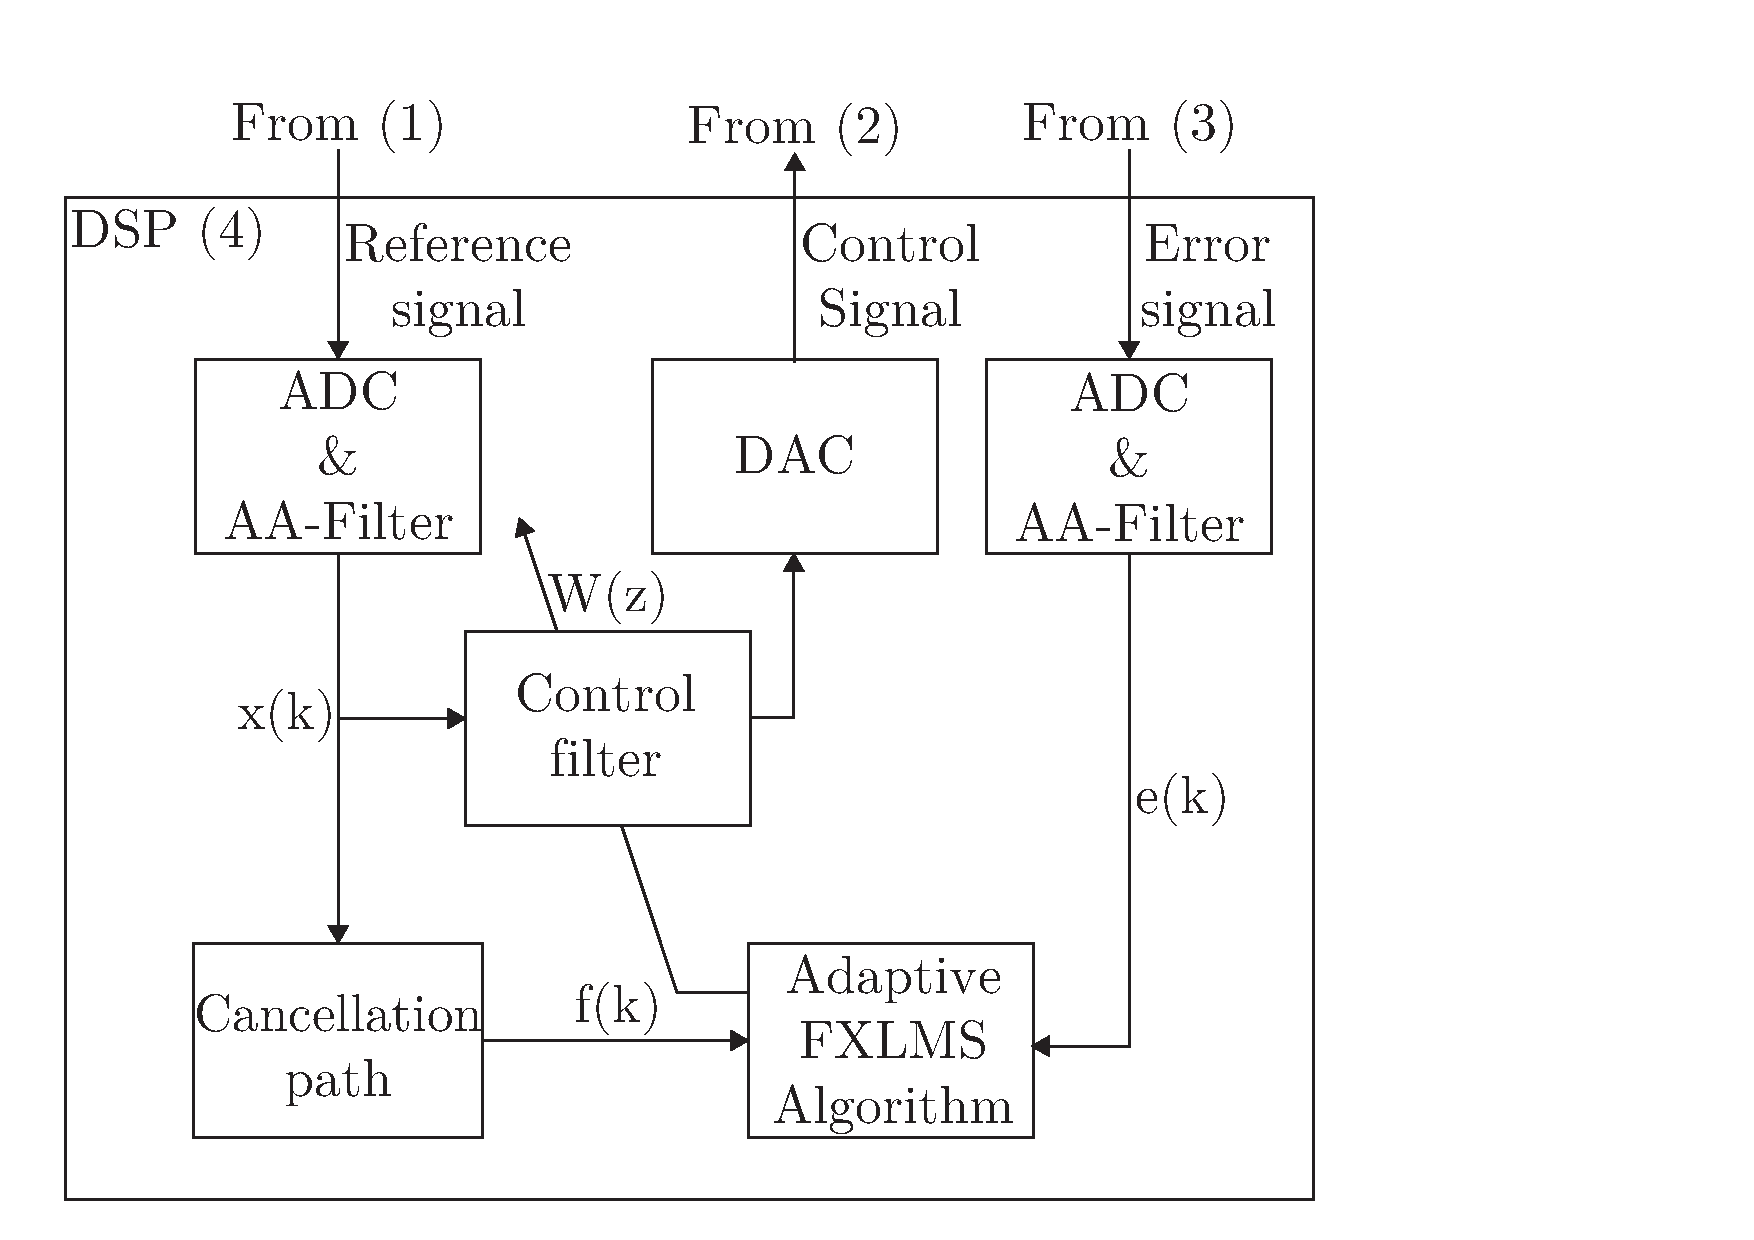
\includegraphics[width=1\columnwidth]{figures/ArticleIllustrations/ANCFeedForward}
%	\caption{Adaptive feedforward ANC system}
%	\label{fig:ANCFeedforward}
%\end{figure}


\textbf{Control Filter} The filter, shown in equation \ref{eq:Output}, is initialized with the inverse of the measured impulse response of the represented transfer function. An order of 256 taps is chosen based on subjective testing in simulation.
\vspace{-3mm} % yeah I know - Sorry Mikkel!
\begin{equation}\label{eq:Output}
y[n]=\sum_{j=0}^{L-1}b_j[n]x[n-j]
\end{equation}
where $b_j[n]$ is the weight coefficients written as  $b[n]=[b_0[n],b_1[n], \cdots, b_{L-1}[n]]^T$.

\textbf{FXLMS} is the optimization algorithm which updates the control filter coefficients using the FXLMS method shown in \autoref{eq:FXLMS}.
\begin{equation}\label{eq:FXLMS}
b_j[n+1] = b_j[n] - 2\mu e[n]f[n-j]
\end{equation}
where $\mu$ is the convergence factor, $e[n]$ is the error and $f[n]$ is the reference convolved with the Cancellation Path.

\textbf{Cancellation Path} (CP) is the transfer-function from the headphone loudspeaker to the error microphone. In the literature \cite{Hansen} the CP is adaptively adjusted, but it is assumed constant because the position of the headphone does not change while measured on a Head and Torso Simulator (HATS). This assumption is made because it is irrelevant for verifying if LP is a plausible solution. 


%When implementing the system, delays exist due to the anti-aliasing and reconstruction filters. The delays of the system exceeds the propagation time of sound from the reference microphone to the headphone loudspeaker resulting in poor performance. Therefore an LP-algorithm is proposed to predict future samples in order to decrease the effect of the time delays.

\subsection{Characteristics of Speech}
Speech can be split into two main classes, voiced and unvoiced. Voiced sounds are characterized by a strong periodicity, with the fundamental frequency referred to as the pitch frequency (50 - 500 Hz). Unvoiced sounds are characterized as random. Speech is a non stationary signal and can only be assumed Wide Sense Stationary (WSS) for periods of 20 - 30 ms \cite{Speech}. 

\subsection{Linear Prediction of Speech}
In order to predict future samples the Auto Correlation Function (ACF), used in LP, of speech must be estimated in frames. The outlines of the prediction system is shown in figure \ref{fig:LinearPredictionOverview}.

\begin{figure}[H]
	\centering
	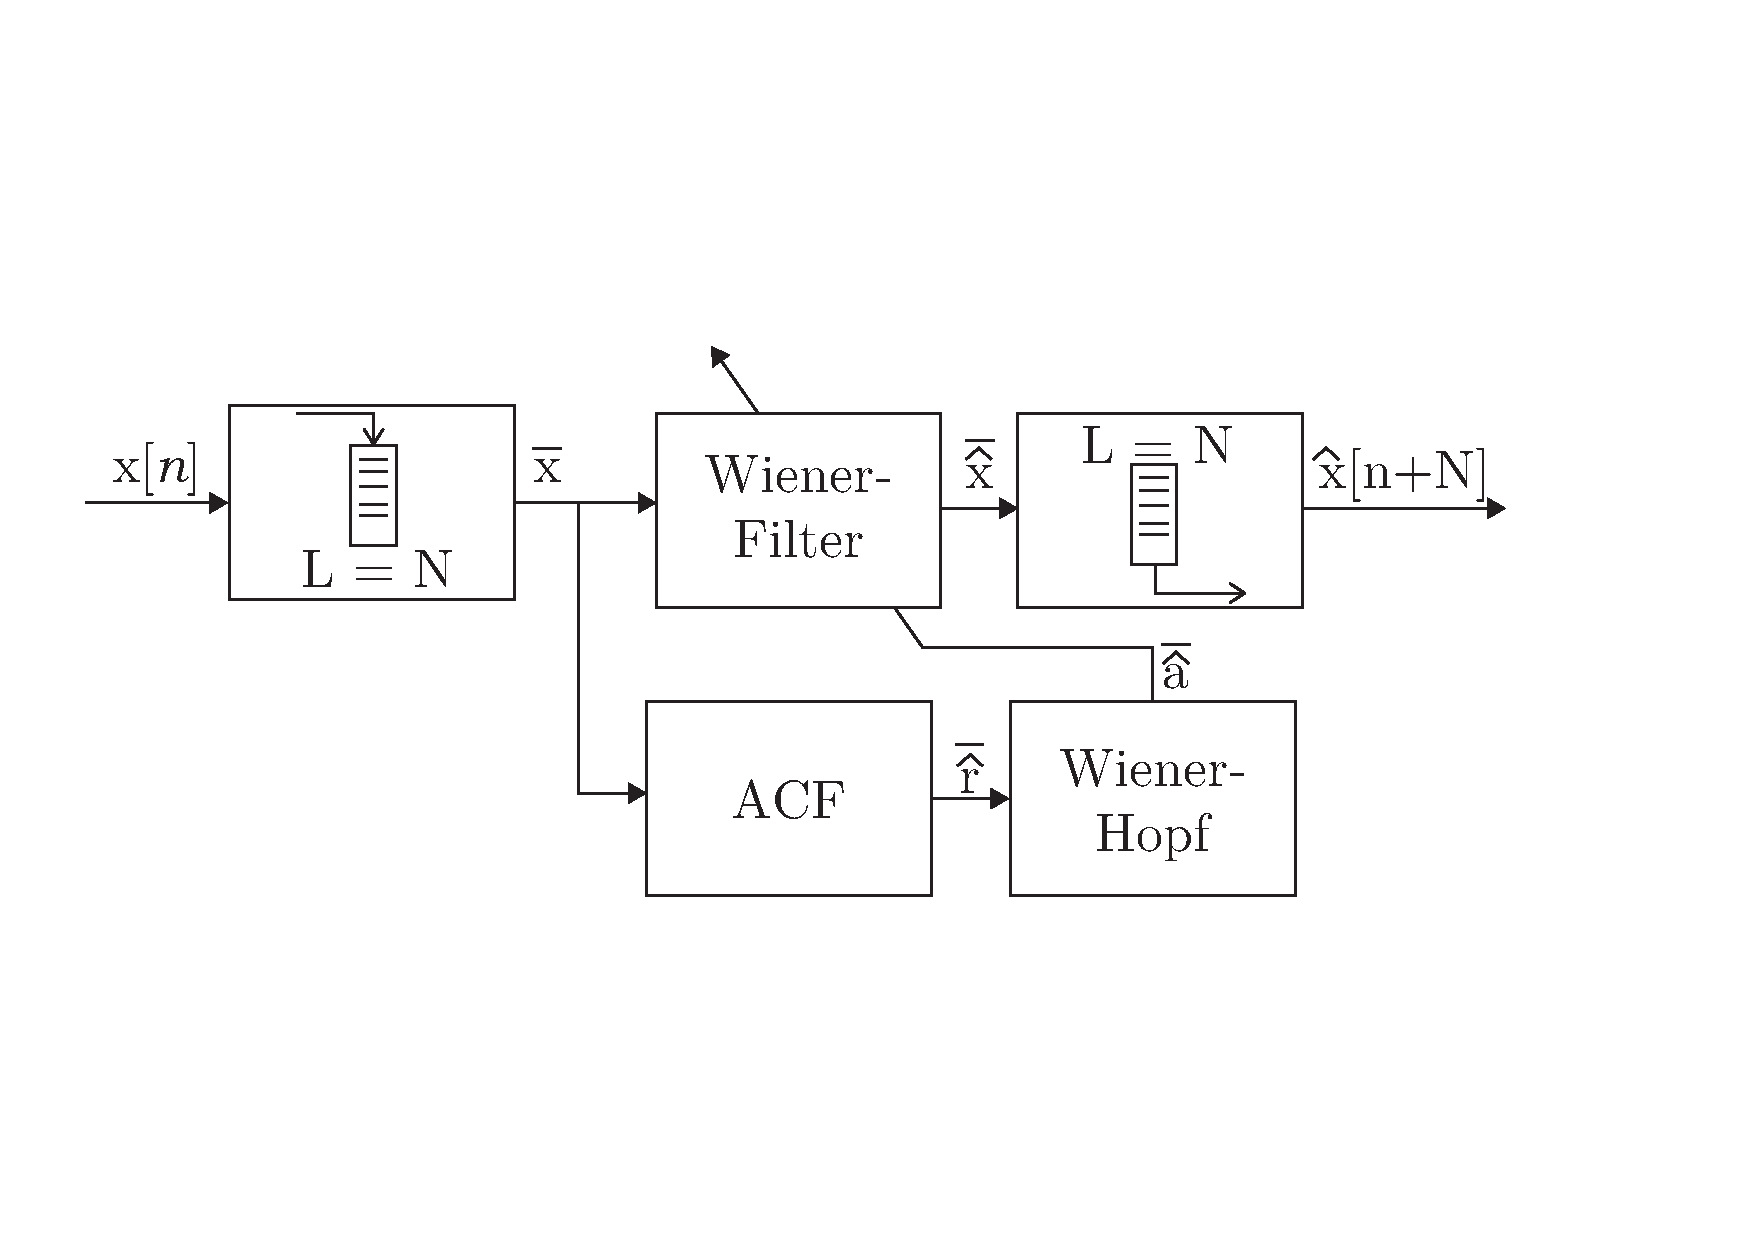
\includegraphics[width=\columnwidth]{ArticleIllustrations/WienerHopf}
	\caption{Linear prediction system.}
	\label{fig:LinearPredictionOverview}
\end{figure}


Utilizing a nonrecursive estimation of the ACF, shown in \autoref{eq:nonrecursive}, it is possible to determine the linear prediction coefficients $\hat{\bar{a}}$ (LPCs) used for predicting future samples \cite{LinearPrediction}. When estimating the ACF of the input ($x$) a Hamming window ($w$) is applied.
\begin{equation}\label{eq:nonrecursive}
%%r_x[l,m] = \sum^{m}_{n=m-N+1+\left| l\right|} x_l[n]w_l[m-n]
\hat{r}_x[l] = \sum^{N}_{n=\left| l\right|} x_l[n]w_l[N-n]
\end{equation}
%\begin{multline}\label{eq:nonrecursive}
%R[l,m] = \sum^{m}_{n=m-N+1+\left| l\right|} \\ x[n]w[m-n] x[n-\left| l\right|]w[m-n+\left| l\right|]
%\end{multline}
%\begin{equation}
%R[l,m]=\sum^{m}_{n=m-N+1+\left| l\right|}x[n]w[m-n] x[n-\left| l\right|]w[m-n+\left| l\right|]
%\end{equation}
where $x_l[n]=x[n]x[n-l]$, $w_l[n]=w[n]w[n+l]$, $l$ is the lag and $N$ is the frame size.

The LPCs are determined using \autoref{eq:normal}, known as the Wiener-Hopf equation.
\begin{equation}\label{eq:normal}
\hat{R}  \bar{a} = -\bar{\hat{r}}_x
\end{equation}
where $\hat{R}$ is the covariance matrix $\hat{C}_{xx}$, $\bar{\hat{a}}$ is the LPCs $\bar{\hat{a}} = [\hat{a}_1 , \hat{a}_2, \cdots, \hat{a}_N]^T$ and $\bar{\hat{r}}_x$ is the ACF, $\bar{\hat{r}}_x = [\hat{r}_x[1] , \hat{r}_x[2], \cdots, \hat{r}_x[N]]^T$.

\autoref{eq:normal} can be rewritten as shown in \autoref{eq:normal2} yielding the LPCs directly.  
 \begin{equation}\label{eq:normal2}
\bar{\hat{a}} = \hat{-R^{-1}} \bar{\hat{r}}_x
\end{equation}
Calculating $\hat{R^{-1}}$ is computationally heavy on a DSP. To estimate the LPCs the Levinson-Durbin method is used \cite{LinearPrediction}. Prediction using Wiener filtering, shown in equation \ref{eq:Predictor}, can then be applied to the current frame for prediction of the next frame. 

\begin{equation}\label{eq:Predictor}
\hat{x}[n+1] =- \sum^{N}_{i=1}\hat{a}_ix[n-i]
\end{equation}

Using equation \ref{eq:Predictor} in cascade where $\hat{x}[n+2]$ is estimated using $\hat{x}[n+1]$ and $x[n]$. The predicted frame is then used as input for the ANC system.

\subsection*{Feedforward LP FXLMS}

